\section{Designing a hybrid place}

Thanks to the development of ubiquitous and pervasive technologies, research focusing on the design of novel interactive artefacts has recently become more concerned with studying and understanding the spatial properties of the world \autocite[p. 159]{hybridplace_ciolfi}. Bringing technologies beyond the desktop and into the world requires an ever-increasing interest in the \emph{physical environment} where interaction occurs \autocite[p. 159]{hybridplace_ciolfi}.  Designing the interaction between ubiquitous technologies and users involves both a re-conceptualization of the interface as an assembly of tangible physical elements (including furniture and everyday objects), and importantly an understanding of the relationship between users and the physical space that is augmented by the technology \autocite[p. 159]{hybridplace_ciolfi}. Following the interest in the physical environment where interaction occurs, Ciolfi and Bannon discusses how geographical notions of space and place can aid designers in creating meaningful interactions between end-users and technologically augmented physical spaces. After reviewing literature that discusses the use of spatial concepts and metaphors within the interaction design field, they present a conceptual frame to design technologically enhanced environments for museums and exhibitions in particular. Their goal is to show how a place-centred approach can practically guide and support design, specifically within a setting that has seen many cases of technology introduction that have led to the visitors' distraction from the museum holdings, instead of extending and supporting the museum experience \autocite[p. 159-160]{hybridplace_ciolfi}.


% They have shown how new information technologies when used in museum environments, often suffer from a number of drawbacks; in particular, they argue that these technologies may hinder visitors appreciation of museum artefacts, their social interaction with others, and their appreciation of the place \autocite[p. 178]{hybridplace_ciolfi}.


Ciolfi and Bannon (2007) are particularly interested in the experience of place. Especially in terms of understanding the ways people come to ascribe meanings to particular places, and how certain places evoke complex webs of significance for people \autocite[p. 160]{hybridplace_ciolfi}. This is different from other similar research approaches that have attempted to use ideas from architecture and urban planning to inform the placement of interactive artefacts, e.g. \autocite{Cullen_book}, or noting how environment affects people's movement and interaction, e.g. \autocite{Alexander_book}. They base their articulation of place on the work of the geographer \autocite{Tuan_book}. According to Tuan, it is only natural that place is grounded in the physical, material reality of the world and that experience is shaped through physical sensing, exploration and habitation. On the basis of Tuan's conceptualisations, Ciolfi and Bannon propose an articulation of the concept of place that highlight the different dimensions as interconnected aspects of the individual experience:


\begin{figure}[H]
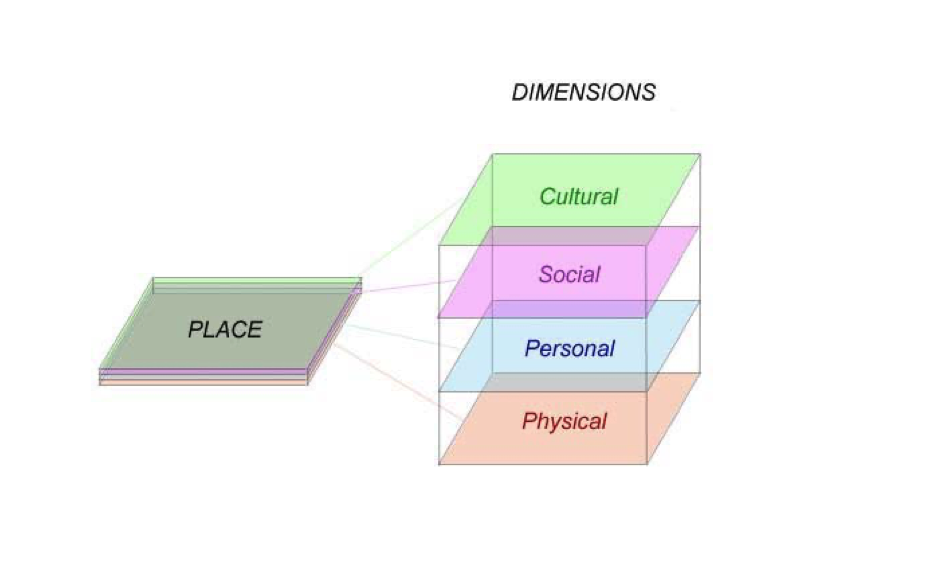
\includegraphics[width=12cm]{pictures/tuans_dimensions.png}
\caption{A representation of Tuans conceptualization of place}
\centering 
\autocite[p. 224]{spaceplace_ciolfi}
\end{figure}

The articulation of the four dimensions of place can help interaction design in interactive spaces by bringing aspects of individual traits and preferences, social interaction and cultural influences together with the physical features of the space \autocite[p. 163]{hybridplace_ciolfi}. These dimensions do not exist \emph{a priori}, but emerge and become visible in practise and experience as they lead to and emerge through peoples actions and activities in the museum space or with the installation \autocite[p. 163]{hybridplace_ciolfi}. As Ciolfi and Bannon explains it, each dimension is present at any moment of one's experience of place, but the experience itself is shaped by the dynamic interconnections among these dimensions. Each particular experience of the place is both individual and unique, although influenced by the presence of- and interaction with others. "Others" could be the other visitors in the museum, or e.g. a group of friends or family visiting together, as is expressed through the social dimension. In order to understand a place and its inhabitants, all four dimensions and their interplay with each other have to be taken into account \autocite[p. 162]{hybridplace_ciolfi}.

% MY OPINIONSSSZZZZZ
\break

Ciolfi and Bannon argue that a place-centred approach can practically guide and support the design of museum experience. I have found this approach helpful when trying to understand how one can design interactive and meaningful museum experiences because it help position and argue for why and how the context e.g. surroundings and environmental qualities influences one's impression of the museum, the exhibition or a particular installation. I believe the concept of a hybrid place can help to understand interaction dynamics in the museum context. In addition to this, it provides a vocabulary and a theoretical lens to talk about and understand a specific experience with e.g. an interactive installation. The level of abstraction on the four dimensions provides an opportunity to incorporate different types of museum experiences. This can be useful in initial stages of a design process when you are getting to know a new museum context, providing a holistic lens to help read the room and learn its truth. 

% \par In my opinion, interactivity alone wont build a meaningful experience, it is a close "samspill" between the installations in the narrative path that the museum build, as well as a way to remember the place where you experienced something meaningful. I believe that over time, when perhaps months or years have passed and the details of the experience is forgotten, what remains is the memory of something meaningful happening in that place; the museum. That's what makes you want to come back to the space, or bring friends and family.


\section{Four dimensions}
When it comes to designing a hybrid place as researched by Ciolfi and Bannon (2007), the main contribution is the place-centred approach that provides the basis for a discussion of the place-related qualities in the museum of study. In Ciolfi and Bannon's case, they used the approach to highlight the limits of existing technologies and to propose the design of novel ones \autocite[p. 163]{hybridplace_ciolfi}, while in my case I am interested in using the place-centred approach to highlight meaningful relations in the museum.

Ciolfi and Bannon conducted a case study - the design of the interactive exhibition 'Re-Tracing the Past' at the Hunt Museum, Limerick - and the study shows how attention to place and its dimensions can inform design in quite concrete ways, and help in overcoming the problems of current interactive museum installations \autocite[p. 178]{hybridplace_ciolfi}. Through their development of their conceptualisation of 'place', involving people's lived experience of the physical space, based on \autocite{Tuan_book}'s work; they articulate four dimensions of place: physical, individual, social and cultural \autocite[p. 178]{hybridplace_ciolfi}. Their evaluations demonstrate that the exhibition they designed supported visitors engagement with museum artefacts, encouraged social interaction, discussion and debate, and allowed for personal and unique contributions to the place \autocite[p. 178]{hybridplace_ciolfi}.

\par
% This is what they did, and what I base my analysis/ lens on 
Through the case study of 'Re-tracing the Past', they derived four dimensions where their consideration of the multiple dimensions of peoples experience allowed to pinpoint issues to be dealt with in the design phase \autocite[p. 178]{hybridplace_ciolfi}.

\begin{itemize}
  \item \emph{The physical/structural dimension:} Relating to materials, structures and environmental factors. The exhibition should be aesthetically pleasing pleasing in order to merge harmonically with the museum; it should should be a space that favours participation and active discovery; it should be welcoming and friendly; it should support group interactions as well as individual's, and be accessible by different age groups.
  \item \emph{The personal dimension.} Related to the feeling and emotions we associate to a place, to the memories related to or evoked by it, to the personal knowledge and background we invest the place with while making sense of it. The exhibition should not have a prescribed sequence of actions in order to allow visitors to configure their visit; the exhibition should encourage visitors to express their opinions, comments and reflections and, to some extent, to leave their own trace; the visitors should feel welcomed and at ease. 
  \item \emph{The social dimension.} Related to social interaction and communication within the place, to the sharing of resources and memories, to social co-ordination and ethics, etc. Social interaction among groups of visitors should be supported and favoured. Also, the museum Docents should be encouraged to take part to the exhibition together with visitors.
  \item \emph{The cultural dimension.} Related to the rules, conventions and cultural identity of a place and of its inhabitants. The exhibition should be a representation of the museum's culture and identity. It should also suggest to visitors that - although located within a museum - the conventional cultural rules of behaviour in museums do not apply to it. People should feel free to interact actively with the installation, make themselves comfortable and so on.
\end{itemize}

% MY OPINIONSSSZZZ 
I intend to use these four dimensions as a foundation for my scope in terms of data-gathering in the different museums and exhibitions that I’m visiting this semester. Ciolfi and Bannon explains how each dimension is present at any moment of one’s experience of a place, and the experience is shaped by the dynamic interconnections among these dimensions(p. 162), and after my museum visits I want to be able to analyse the museums and be enabled to identify some interconnections between the physical, personal, social and cultural dimension in a museum. I also intend to use the four dimensions in the synthesising of the framework of how to design meaningful interactive museum experiences.

\break
Their consideration of the multiple dimensions of people's experience allowed to pinpoint issues to be dealt with in the scenario design phase \autocite[p. 178]{hybridplace_ciolfi}, which are as following:

\autocite[p. 168]{hybridplace_ciolfi} articulate four pitfalls or "problems" that arise: 
\begin{itemize}
    \item How people appreciate the exhibit
    \item How people interact with eachother; and
    \item How people devise their own path through the exhibits and leave a trace of their presence in the space.
\end{itemize}


\section{Place-related qualities of a hybrid museum}

The perspective of “Ubiquitous Computing”, proposed in the early 1990’s by Mark Weiser, is based on technological developments that make it possible to embed powerful computational elements and digital components into everyday objects, portable devices and the built environment. This trend is inducing significant changes not only in the development and implementation of new technology, but also, and more interestingly, on the relationship between interactive systems and their users. \autocite[p. 217]{ciolfi_space_2005}. Design must now concern itself rather with the physical environments that people will experience through their daily lives. People will encounter technologically enhanced spaces and artefacts as they move through a variety of environments \autocite[p. 217]{ciolfi_space_2005}. These systems will change the way in which physical spaces are used and shaped by people, where the systems are able to react and respond to their presence and actions. The activities of interacting with the space and its elements and interacting with the computer system will merge into each other \autocite[p. 217]{ciolfi_space_2005}. 

The Interaction Design field is currently ongoing a shift in the understanding of the relationship between people and technologies, where HCI primarily have been focused on a single users individual traits and preferences to computer functionalities and interface elements, a one-to-one relationship with the computer system. Interaction Design is also corned with the role of social, emotional and contextual factors in influencing human interaction with a computer system \autocite[p. 217]{ciolfi_space_2005}.

Context-aware systems are those that are able to sense features of the physical setting, and to feed a representation of this data into the system itself. The sensing devices can be located both around the physical environment and on the bodies of the inhabitants \autocite[p. 218]{ciolfi_space_2005} An example of an enhanced space is that of “Narrative Spaces” (Sparacino 2002), where users are able to produce “augmented” performances on an interactive stage with the support of sensors and gesture modeling tools: the performers physical movements trigger the production of sounds and computer-generated images on large display screens\autocite[p. 219]{ciolfi_space_2005}. 

Ciolfi and Bannons research aim to apply the concept of place to a particular set of ubiquitous systems: technologically-enhanced physical spaces. With ubiquitous technologies becoming more reliable and widespread, we are now dealing with fully interactive physical spaces, containing tangible elements acting as interfaces to access features of the digital domain. We believe, as noted by Ciolfi and Bannon, the concept of place can assist interaction designers to understand interaction dynamics in this context, and to propose effective design concepts: where place goes beyond the vision of space just as a physical setting, a container, and includes many dimensions of human experience within an environment\autocite[p. 221]{ciolfi_space_2005}.
